\section{Architecture}
The central classes of our game handle theming, player actions, game logic 
and the graphical representation of the game. These central
classes of our game are depicted in Fig.\ref{fig:architecture}.
%
The first instantiated class is FBGame. FBGame controls some of the global 
game functionality, like the number of players, reward strategies like 
highscores and the conditions of victory and defeat. It is also responsible 
for instantiating the FBWorld class which encapsulates graphical 
representation of the game.

FBWorld is passed a symbol at startup, which is the name of a FBTheme. FBWorld 
holds a reference to the current theme and creates its main submorphs, like
a menu, highscore list the changing backgrounds and the in-game playfields.
These Morphs, however, are not held in an instance variable of any kind, but 
are returned to the FBGame instance, for co-ordination.\\
Out of technical necessity, FBWorld also catches all keystrokes, handling them, 
however, is up to the FBGame. Global events, like pause and quit, are handled 
directly, all other keystrokes are passed on to all playfields in the game (if any)
and handled there.

FBPlayfields are created by the world upon the requirements of the theme
and then returned to the FBGame. The playfields receive their own reference 
to the theme and are themselves responsible for their content and reaction on 
player input, thus allowing us to implement multiplayer gaming simply by creating 
more playfields in our world.
%
\begin{figure}[bt]
  \begin{center}
    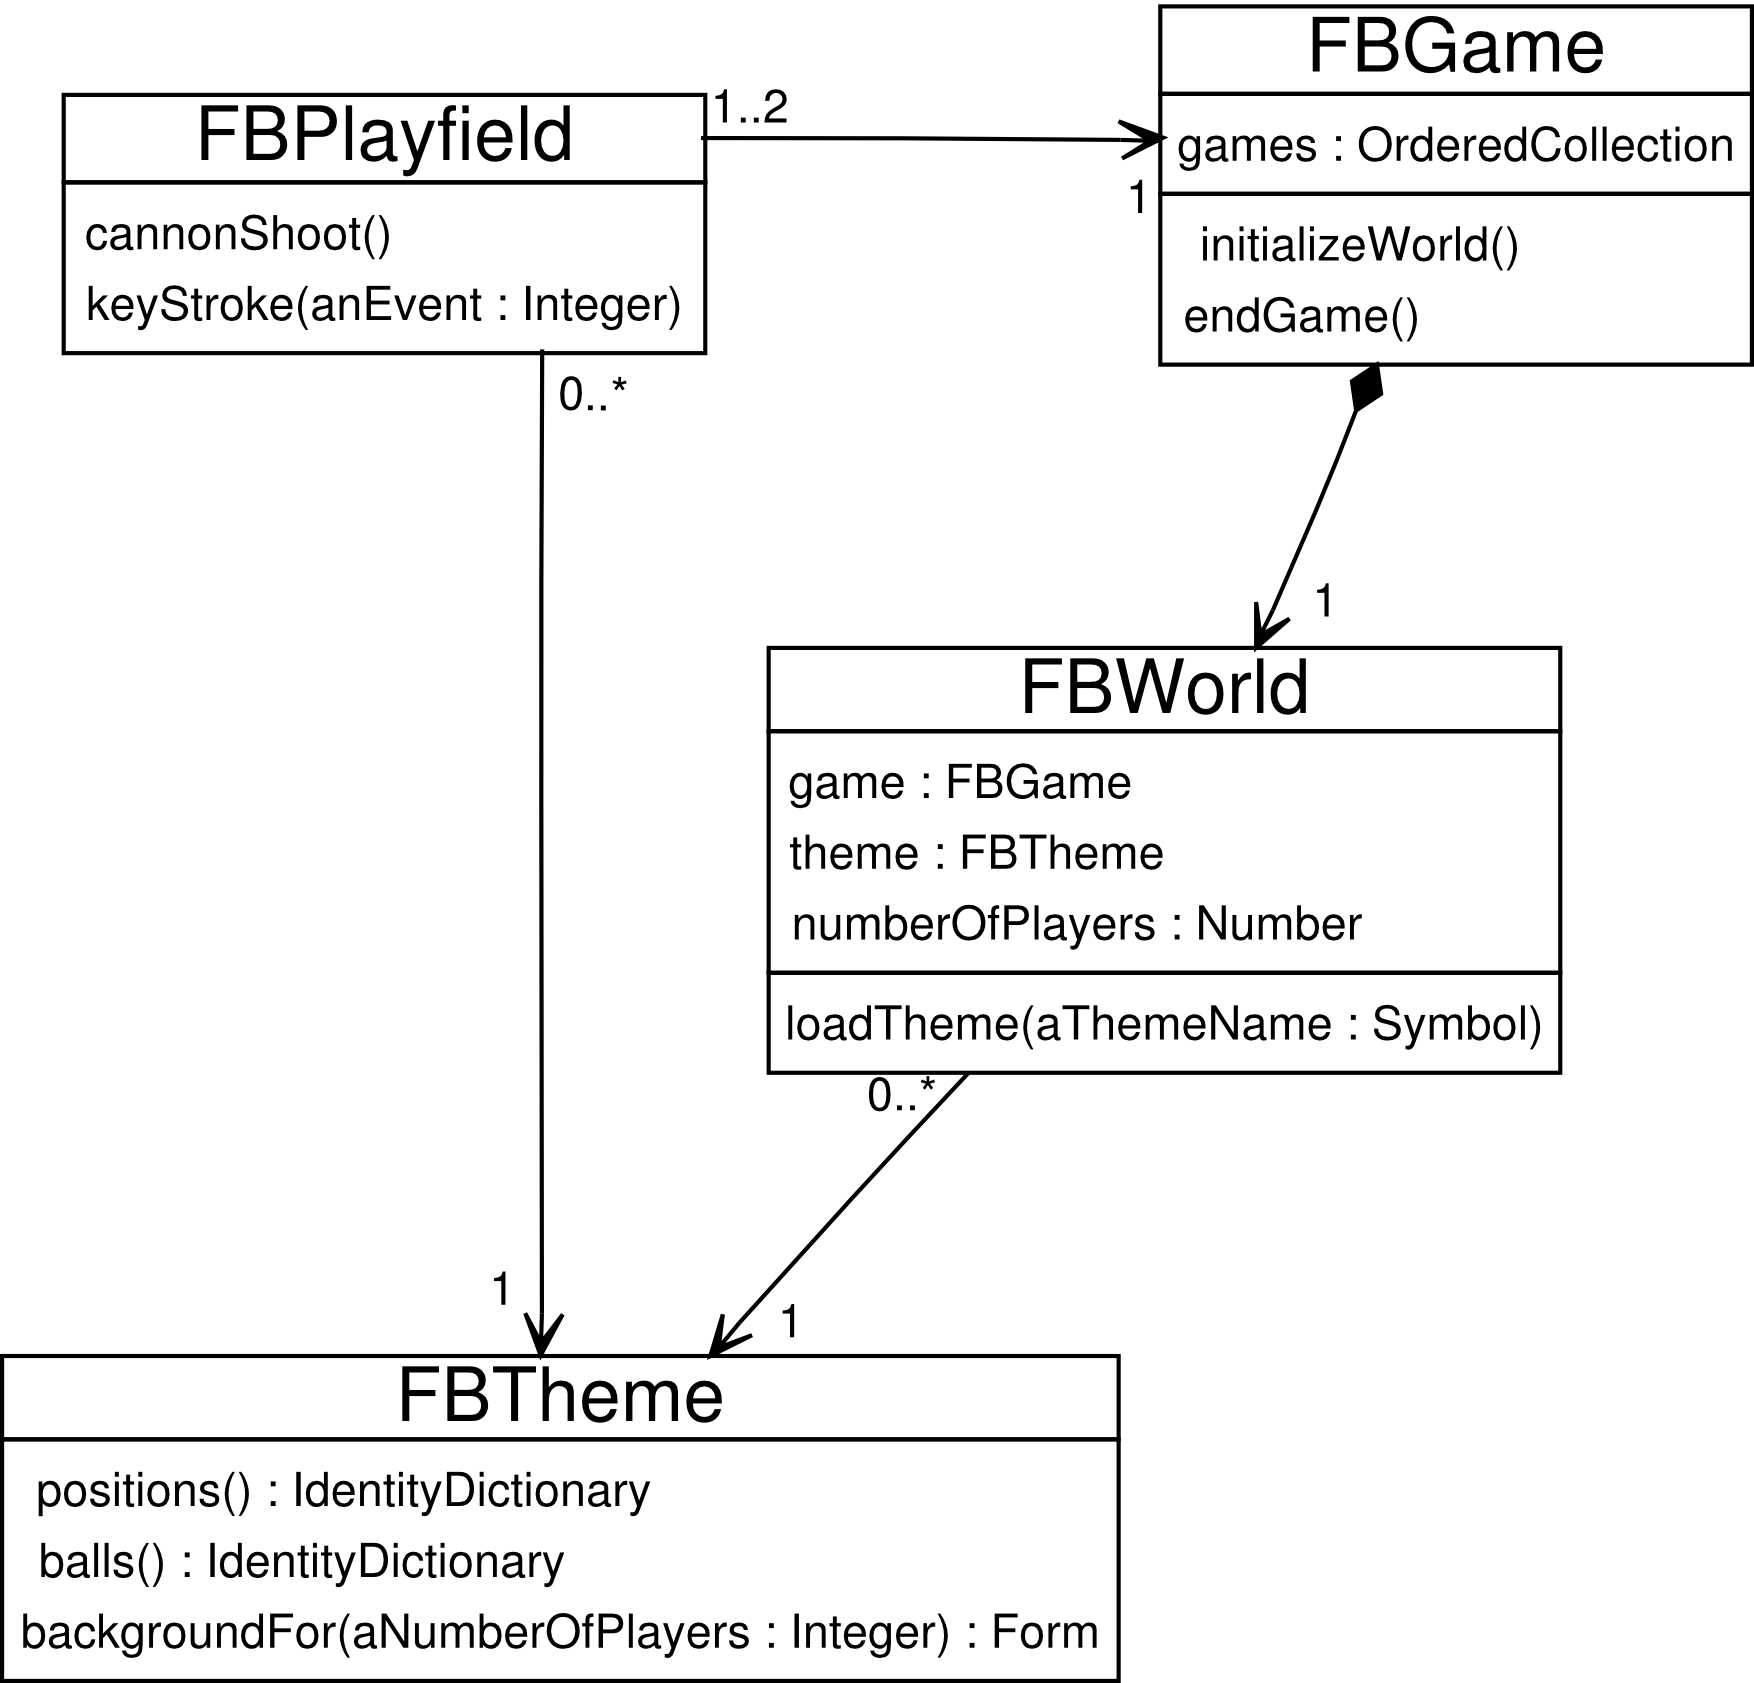
\includegraphics[width=0.6\linewidth]{images/architecture.png}
  \end{center}
  \caption{The Central System Architecture}
  \label{fig:architecture}
\end{figure}


